\documentclass[10.7pt,]{article}

\usepackage[letterpaper, margin=2.54cm, top=2.54cm]{geometry}
\usepackage[super,comma,sort&compress]{natbib}
\usepackage{lmodern}
\usepackage{authblk} % To add affiliations to authors
\usepackage{amssymb,amsmath}
\usepackage{wrapfig}
\usepackage{graphicx,grffile}
\usepackage[labelfont=bf,labelsep=period]{caption}
\usepackage{ifxetex,ifluatex}
\usepackage{fixltx2e} % provides \textsubscript
\ifnum 0\ifxetex 1\fi\ifluatex 1\fi=0 % if pdftex
  \usepackage[T1]{fontenc}
  \usepackage[utf8]{inputenc}
\else % if luatex or xelatex
  \ifxetex
    \usepackage{mathspec}
  \else
    \usepackage{fontspec}
  \fi
  \defaultfontfeatures{Ligatures=TeX,Scale=MatchLowercase}
    \setmainfont[]{Times New Roman}
    \setsansfont[]{Century Gothic}
    \setmonofont[Mapping=tex-ansi]{Consolas}
\fi
% use upquote if available, for straight quotes in verbatim environments
\IfFileExists{upquote.sty}{\usepackage{upquote}}{}
% use microtype if available
\IfFileExists{microtype.sty}{%
	\usepackage{microtype}
	\UseMicrotypeSet[protrusion]{basicmath} % disable protrusion for tt fonts
}{}

\usepackage{lipsum} % for dummy text only REMOVE

\newtheorem{exm}{Example}


%==============================
% Customization to make the output PDF 
% look similar to the MS Word version
%==============================
% To prevent hyphenation
\hyphenpenalty=10000
\exhyphenpenalty=10000

% To set the sections font size
\usepackage{sectsty}
\allsectionsfont{\fontsize{10}{10}\selectfont}
%\sectionfont{\fontsize{10}{10}\selectfont}
\subsectionfont{\itshape\bfseries\fontsize{10}{10}\selectfont}
\subsubsectionfont{\normalfont\itshape}

% No new line after subsubsection
\makeatletter
\renewcommand\subsubsection{\@startsection{subsubsection}{3}{\z@}%
	{-3.25ex\@plus -1ex \@minus -.2ex}%
    {-1.5ex \@plus -.2ex}% Formerly 1.5ex \@plus .2ex
    {\normalfont\itshape}}
\makeatother

\makeatletter % Reference list option change
\renewcommand\@biblabel[1]{#1.} % from [1] to 1
\makeatother %

% To set the doc title font
\usepackage{etoolbox}
\makeatletter
\patchcmd{\@maketitle}{\LARGE}{\bfseries\fontsize{15}{16}\selectfont}{}{}
\makeatother

% No page numbering
\pagenumbering{gobble}

\makeatletter
\def\maxwidth{\ifdim\Gin@nat@width>\linewidth\linewidth\else\Gin@nat@width\fi}
\def\maxheight{\ifdim\Gin@nat@height>\textheight\textheight\else\Gin@nat@height\fi}
\makeatother

% Scale images if necessary, so that they will not overflow the page
% margins by default, and it is still possible to overwrite the defaults
% using explicit options in \includegraphics[width, height, ...]{}
\setkeys{Gin}{width=\maxwidth,height=\maxheight,keepaspectratio}
\setlength{\parindent}{0pt}
\setlength{\parskip}{6pt plus 2pt minus 1pt}
\setlength{\emergencystretch}{3em}  % prevent overfull lines
\providecommand{\tightlist}{%
  \setlength{\itemsep}{0pt}\setlength{\parskip}{0pt}}
\setcounter{secnumdepth}{0}
% Redefines (sub)paragraphs to behave more like sections
\ifx\paragraph\undefined\else
\let\oldparagraph\paragraph
\renewcommand{\paragraph}[1]{\oldparagraph{#1}\mbox{}}
\fi
\ifx\subparagraph\undefined\else
\let\oldsubparagraph\subparagraph
\renewcommand{\subparagraph}[1]{\oldsubparagraph{#1}\mbox{}}
\fi
%==============================
\usepackage{hyperref}
\hypersetup{
	unicode=true,
	pdftitle={Understanding prediction model generalization through the lens of causality},
	pdfauthor={Su Li},
	pdfkeywords={keyword1, keyword2},
	pdfborder={0 0 0},
	breaklinks=true
}
\urlstyle{same}  % don't use monospace font for urls
%==============================

% reduce space between title and begining of page
\title{\vspace{-2em} Understanding prediction model generalization through the lens of causality}
\author[ ]{\bf\fontsize{13}{14}\selectfont Su Li, Master's Student\textsuperscript{1}\vspace{-.7em}}
\affil[1]{\bf\fontsize{13}{14}\selectfont Faculty of Social and Behavioural Sciences, Utrecht University, Netherlands}
\date{}


%==============================
\begin{document}
\maketitle
\vspace{-4em} %separation between the affiliations and abstract
%==============================



%==============================
\section{Introduction}\label{introduction}
%==============================
Prediction models are widely used in medical domains and settings to help doctors detect whether the patients suffer from a particular disease (diagnosis) or to predict the occurrence of a specific outcome (prognosis).\cite{1,2} Thus, robust model performance is essential for generating reliable and accurate decisions. However, no model is robust across different environments; models’ performance may differ when evaluated in datasets that are not used to develop the model.\cite{3} For example, university hospitals usually serve more severe cases than primary care physicians. So, a model based on university hospitals may perform worse in primary care physicians. In the healthcare area, this kind of change in patient distribution can be described as a change in ‘case-mix’.\cite{4}  

Recently, the definition of ‘case-mix’ has been interpreted differently within the causal inference framework. In diagnostic prediction models, we typically predict the underlying diagnosis (\(Y\)) based on the symptoms (\(X\)). In this case, the underlying diagnosis serves as the cause, and symptoms are the effect, meaning the model predicts the cause from the effect. In this context, diagnostic prediction models follow an \textbf{anti-causal direction}. The case mix here is interpreted as a change in the marginal distribution of the diagnosis. In contrast, we typically predict the future outcome (\(Y\)) based on the current patient characteristics (\(X\)) in prognostic models. Patient characteristics can be seen as the cause, and the future outcome is the effect. Thus, the prediction direction here follows a \textbf{causal direction}. The case mix refers to the distribution of patient characteristics.

  
Calibration and discrimination are the two traditional predictive performance metrics.\cite{3} Discrimination measures how well the model distinguishes the positive and negative cases, while calibration refers to the agreement between predicted and observed probability.\cite{5} As demonstrated by Van Amsterdam,\cite{6} calibration tends to remain stable in causal direction prediction (prognostic), while discrimination remains consistent in anti-causal direction predictions (diagnostic) under shifts in case-mix. This is because discrimination relies on the distribution of features conditioned on the outcome (\(X \mid Y\)), making it independent of changes in the marginal distribution of the outcome. Meanwhile, calibration depends on the outcome given the features (\(Y \mid X\)) and thus remains unchanged under the shifts of the marginal distribution of the features.

This study aims to use empirical analysis to validate that calibration remains stable for the causal-direction models. In contrast, discrimination remains stable for anti-causal models under shifts in case mix. If validated, this theory could help us understand the varying performances of different prediction models (prognostic and diagnostic) across diverse environments, guiding the selection of appropriate evaluation metrics. For prognostic models, changes in discrimination are expected when case-mix shifts across different settings, while calibration should remain stable. When evaluating diagnostic models’ performance across various settings, changes in calibration are expected, but changes in discrimination are not. Meanwhile, depending on the aim of the task and the prioritization of either discrimination or calibration, model developers can choose to use entirely causal or entirely anti-causal variables to enhance the robustness of prediction models under shifts in case mix.

The eICU dataset is used to evaluate the hypothesis empirically across multiple environments. Several prognostic and diagnostic prediction models are developed using logistic regression, and their performances are assessed by discrimination and calibration across different training and test sets. The Results section presents descriptive statistics and the preliminary results, and  the Discussion section summarizes the current results and outlines future plans.



%==============================
\section{Methods}\label{methods}
%==============================

%==============================
\subsection{Data sources}\label{data-sources}
%==============================

In this study, the eICU Collaborative Research Database (version 2.0) \cite{7} will be used, which is a publicly available, multicenter database containing de-identified data on 200,859 ICU patients from 208 hospitals across the United States from 2014 to 2015 \cite{8}. This database includes detailed records on patient demographics, vital sign measurements, diagnosis information, treatment information, laboratory results, and outcomes such as mortality. Three variables can be used to split the dataset to create different clusters: \texttt{hospital\_region}, \texttt{hospital\_bed\_size}, and \texttt{hospital\_teaching\_status}.

\begin{itemize}
    \item \textbf{\texttt{Hospital Region}} clusters the 208 hospitals based on their geographical location (Midwest, Northeast, South, West, Unknown (those are missing in hospital region value)).
    \item \textbf{\texttt{Hospital Bed Size}} categorizes hospitals by their capacity (\(<100\) beds, 100--249, 250--499, \(\geq500\), Unknown).
    \item \textbf{\texttt{Hospital Teaching Status}} indicates whether the hospital is a teaching institution or non-teaching.
\end{itemize}


%==============================
\subsection{Analysis Methods}\label{Analysis Methods}
%==============================

Logistic regression (LR) is a widely used method to analyze the relationship between predictors (independent variables) and dichotomous outcomes (dependent variable). Since logistic regression is already well-calibrated and well-discriminated, we use it to verify that calibration remains invariant for prognostic prediction models while discrimination remains stable for diagnostic prediction models under shifts in case mix.

Calibration evaluates how well predicted probabilities agree with observed outcome proportion. A prediction model is said to be calibrated when the predicted risks are consistent with the observed proportions of the event. In this study, calibration error is measured with the smooth expected calibration error.\cite{9} Discrimination refers to how well the model can separate between positive and negative cases. Discrimination is evaluated using the area under the curve (AUC). A score close to 1.0 indicates perfect discrimination, while near 0.5 suggests no discrimination.\cite{10} 


%==============================
\subsection{Research Design}\label{Research Design}
%==============================

We will define several prediction tasks that can be classified either as prognosis (e.g. 30-day mortality) or diagnosis (e.g. underlying diagnosis ICU admission). Independent variables will be selected based on previous literature and expert recommendations, taking particular notice of whether the independent variables are causal of the outcome (in the case of prognosis), anti-causal (in the case of diagnosis), or neither. Observations with missing values in the outcome variables were removed from the dataset. For numerical variables, missing values will be imputed by their mean, while for categorical variables, missing values will be imputed by the value with the most frequency. We will split the dataset based on the variables \texttt{hospital\_region}, \texttt{hospital\_bed\_size}, and \texttt{hospital\_teaching\_status}, selecting one subgroup as the training set, while the remaining subgroups will form the test sets. This process will repeat across all subgroups.
  
For each task and each testing hospital, we will record the difference in AUC ($\delta$-AUC) and calibration error ($\delta$-ECE) between the training fold ($\text{AUC}_0 / \text{ECE}_0$) and the testing fold ($\text{AUC}_1 / \text{ECE}_1$). To ensure comparability across subgroups and tasks, $\delta$-AUC and $\delta$-ECE will be standardized by their values in the training fold. According to the causal-case mix hypothesis, prognostic models are expected to maintain calibration across external validation under shifts in case-mix, while for diagnostic models, the discrimination remains the same. To evaluate these differences, we will use an F-test to compare whether the variances of $\delta$-AUC and $\delta$-ECE differ significantly between prognostic and diagnostic models. Specifically, we sum up the variances of $\delta$-AUC (or $\delta$-ECE) for prognostic and diagnostic models separately. Then, the F-test is used to test the null hypothesis that the variances of prognostic models are the same as those of diagnostic models. 
  
\[
\delta = \frac{(\text{AUC}_1 - 0.5) - (\text{AUC}_0 - 0.5)}{(\text{AUC}_0 - 0.5)}
\]
  
Taking discrimination as an example, diagnostic models are expected to have stable discrimination scores. So, the differences in discrimination between the training set and testing set for diagnostic models are expected to be 0. Thus, $\text{VAR}(\delta_{\text{diagnostic}})$ is also anticipated to be 0. While for prognostic models, discrimination scores are expected to vary between training and testing sets. Therefore, $\text{VAR}(\delta_{\text{prognostic}})$ is anticipated to be statistically significantly larger than the variances of diagnostic models.





%==============================
\section{Results}\label{results}
%==============================
\subsection{Descriptive Analysis}\label{Descriptive Analysis}
So far, three tasks have been built: mortality (prognosis), age (diagnosis), and gender (diagnosis). The variables were selected according to the article by Tang et al.,\cite{11} which selected variables based on several evaluation scores that are often used in ICU: SOFA, SAPs, APACHE II, and APACHE IV. The mortality model is a prognostic model that predicts whether the patient in the ICU survived (0) or died (1). Age and Gender are used as diagnostic models. Age is categorized by the median value (64 years), with age \(\geq\) 64 as 1 and age < 64 as 0. Gender is coded as male is 1 and female is 0.
  
Table ~\ref{tab:Table1} shows the sample size and positive case counts together with their percentages for mortality across different hospital characteristics: region, bed size, and teaching status. Using the mortality task as an example, it is evident from the table that the mortality rates vary significantly across different regions. The Northeast region has the lowest number of samples (9071, 6.92\%) but the highest mortality rate (11.98\%). However, the Midwest region has the largest sample size (44879, 34.25\%) with the lowest mortality rate (7.8\%). The South region has a relatively high sample size (42265, 32.25\%) with a mortality rate of 9.98\%. The West and Unknown have similar mortality rates of 8.93\% and 8.27\%, respectively. The rate of Unknown somewhat indicates the average mortality rate of all the groups. Subgroups categorized by \texttt{hospital\_bed\_size} show that both the sample size and mortality rate decrease as the number of beds reduces. Hospitals with more than 500 beds have the largest sample size (50303, 38.38\%) and the highest mortality rate (10.26\%), while those with smaller than 100 beds show the smallest sample size (7301, 5.57\%) and the lowest mortality rate (6.7\%). Teaching hospitals have a higher mortality rate (9.8\%) compared to non-teach hospitals (8.76\%).


\begin{table}[ht]
\centering
\caption{Distribution of Sample and Positive Case Counts by Hospital Characteristics.}
\resizebox{0.7\textwidth}{!}{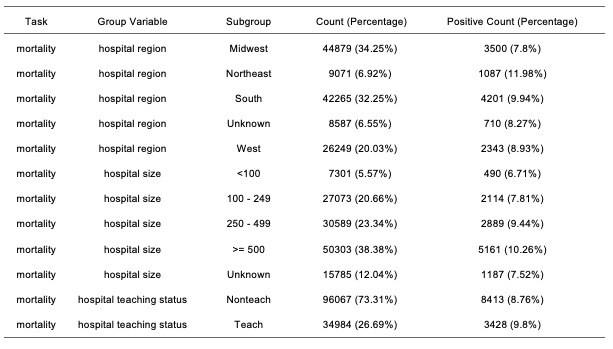
\includegraphics{./figures/descriptive-table.png}}  
\label{tab:Table1}
\end{table}

\subsection{Prediction Performance Across Hospital Characteristics}\label{Prediction Performance Across Hospital Characteristics}

The figures (Figure~\ref{fig:figure1}, Figure~\ref{fig:figure2}, and Figure~\ref{fig:figure3}) illustrate the calibration error (x-axis) and discrimination (AUC, y-axis) for the three tasks across subgroups grouped by \texttt{hospital\_region}, \texttt{hospital\_bed\_size}, and \texttt{hospital\_teaching\_status}. The arrows start from the training set's performance to the test sets' performance. Different line styles correspond to different tasks, while symbols and colors represent subgroups and training environments, respectively. For the mortality task with the Midwest group as the training set, the arrows start at the training performance and spread to the test groups. The movements show a decline in performance, indicating increased calibration error and lower discrimination scores.

Across all groups, mortality prognosis models consistently show low and stable calibration errors, indicating that the prognostic model is well-calibrated. While AUC varies slightly (0.73-0.78), calibration performance remains stable across subgroups. In Figure~\ref{fig:figure1}, calibration errors stay near 0 for most training regions and show a slightly minimal increase when tested on others. Similarly, in Figure~\ref{fig:figure2} and Figure~\ref{fig:figure3}, calibrations remain stable, confirming the reliability of these models.

In contrast, diagnostic models for age and gender result in low discrimination (AUC $\sim$ 0.5-0.65), suggesting weak discrimination ability. In Figure~\ref{fig:figure2} and Figure~\ref{fig:figure3}, changes in calibration errors are minimal ($<$ 0.06), but show clear variations compared to the values of prognostic models in the same group.


\begin{figure}[ht]
\centering
\begin{minipage}{\textwidth}
  \centering
  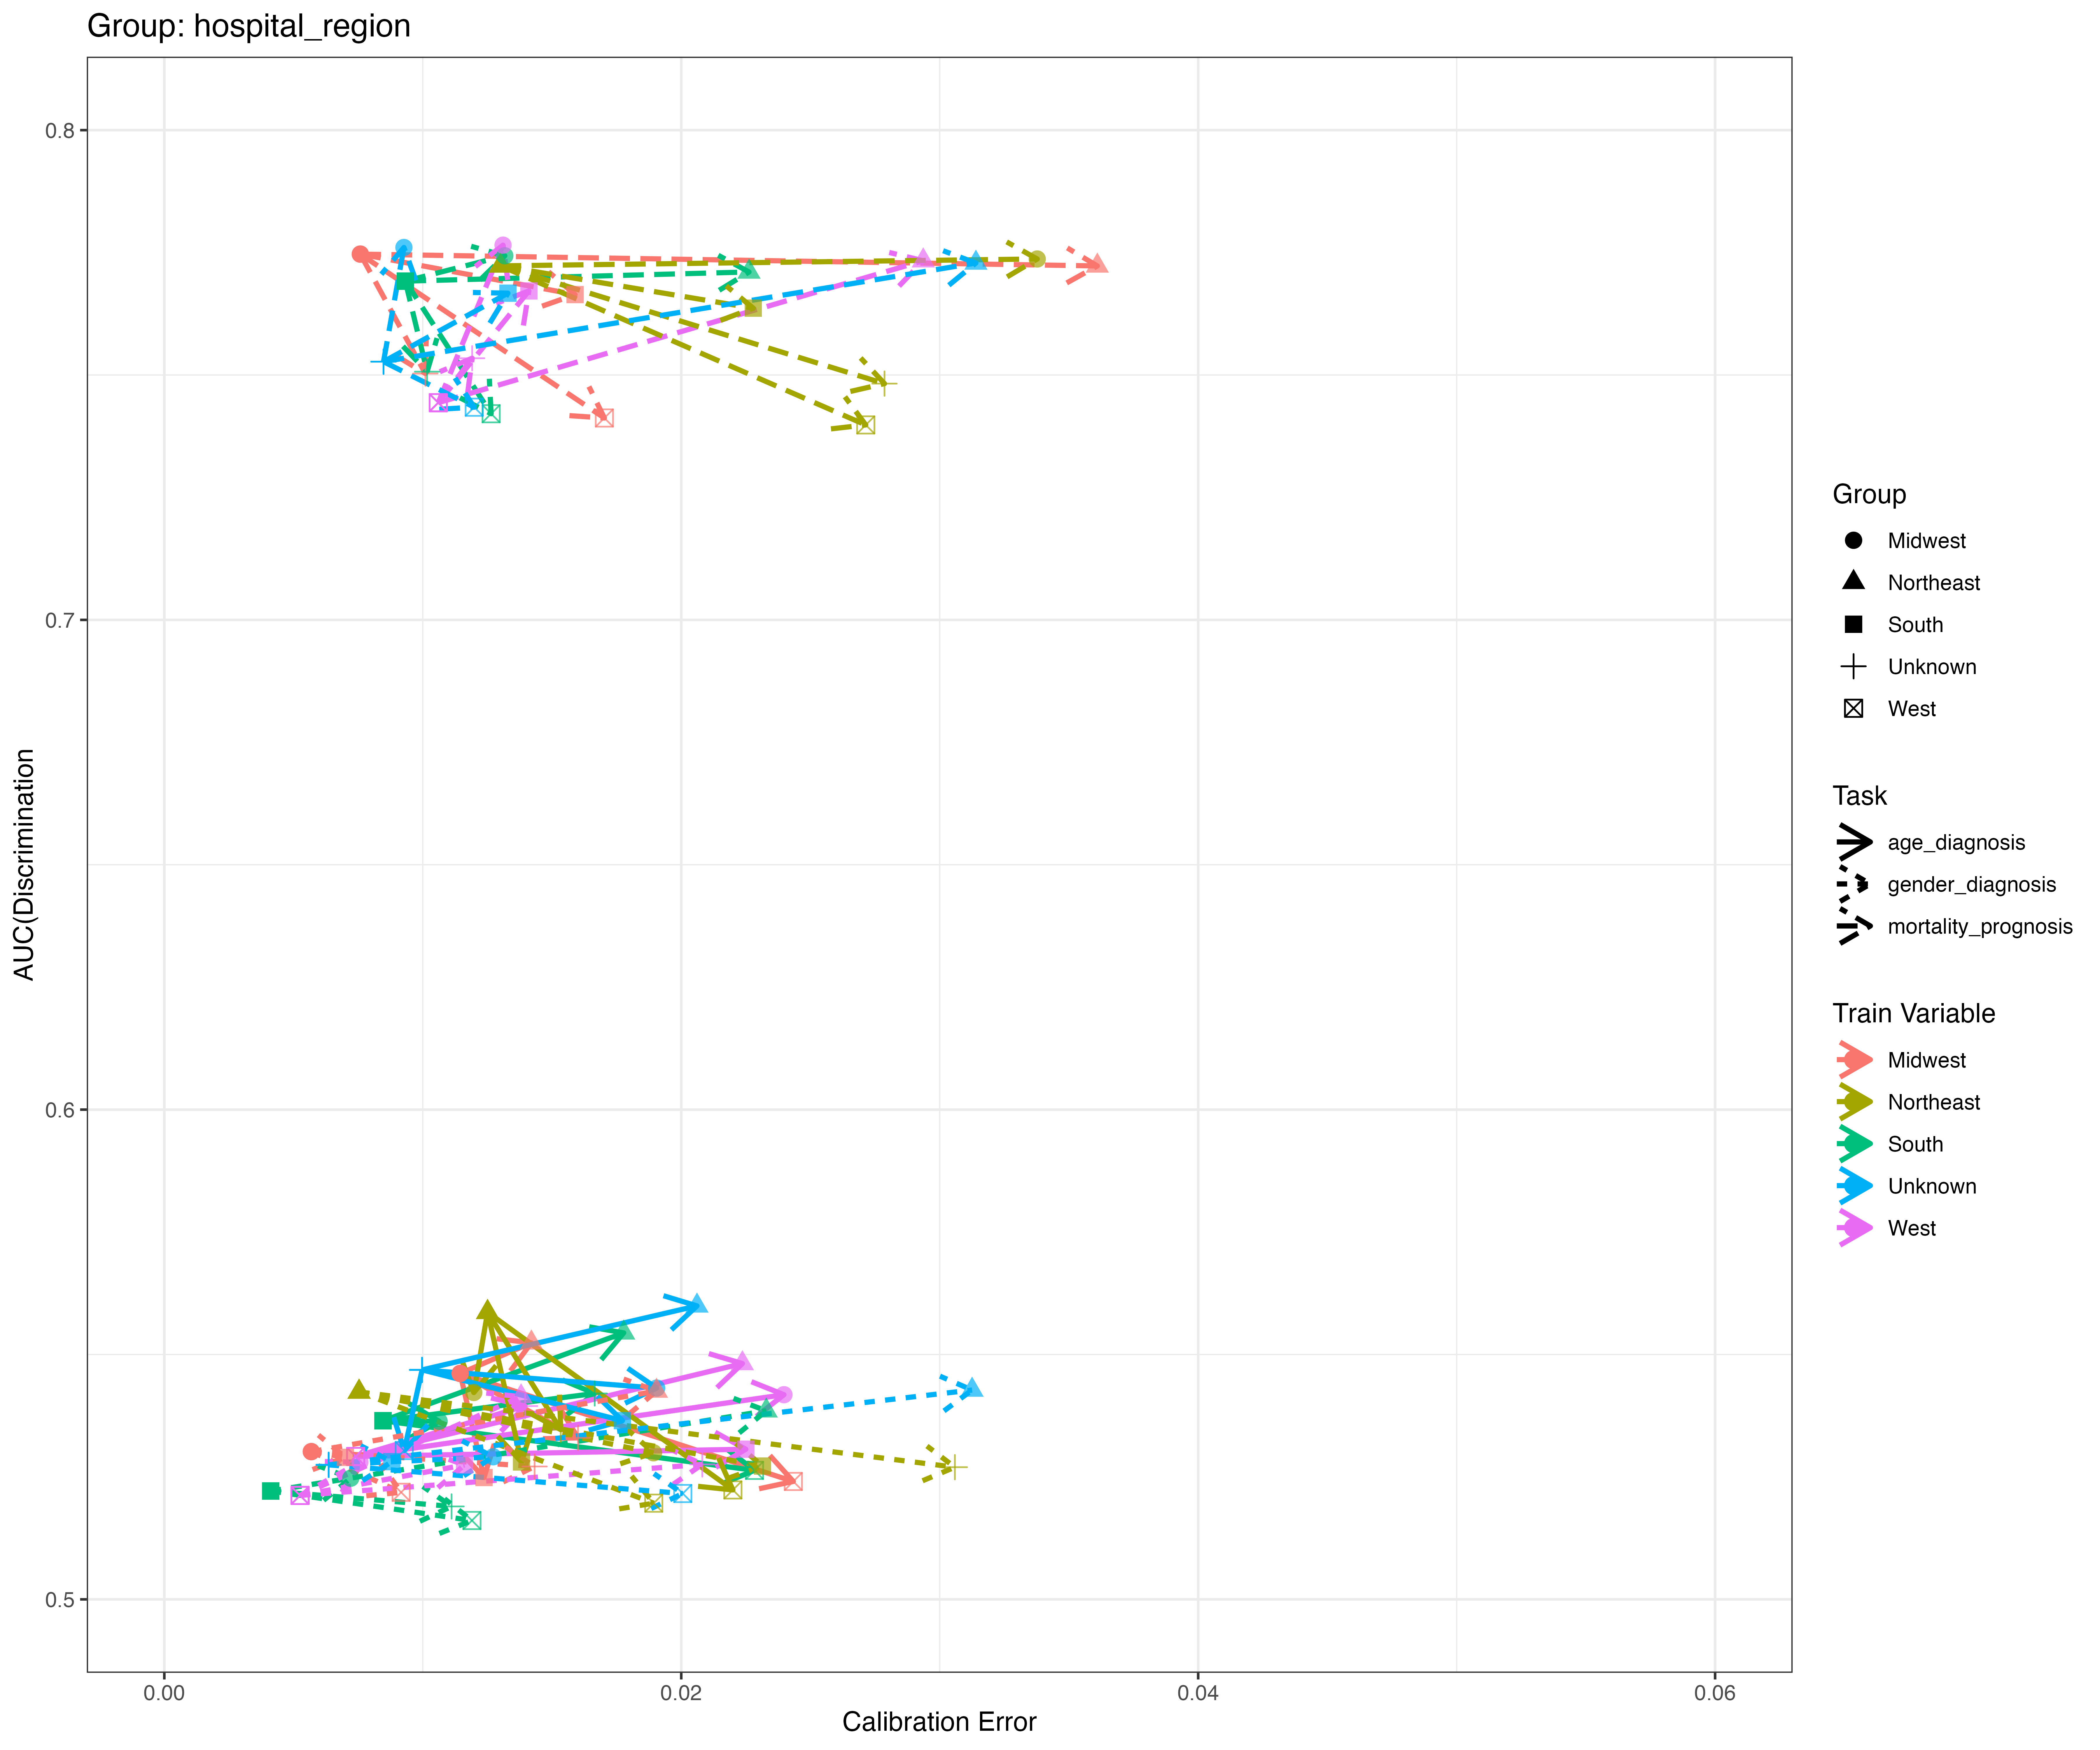
\includegraphics[height=0.45\textheight]{./figures/figure1.png}  % 图像2,设置高度
  \caption{Discrimination vs. Calibration Error Across Hospital Regions and Tasks.}
  \label{fig:figure1}
\end{minipage}
\end{figure}

\newpage
\begin{figure}[ht]
\centering
\begin{minipage}{\textwidth}
  \centering
  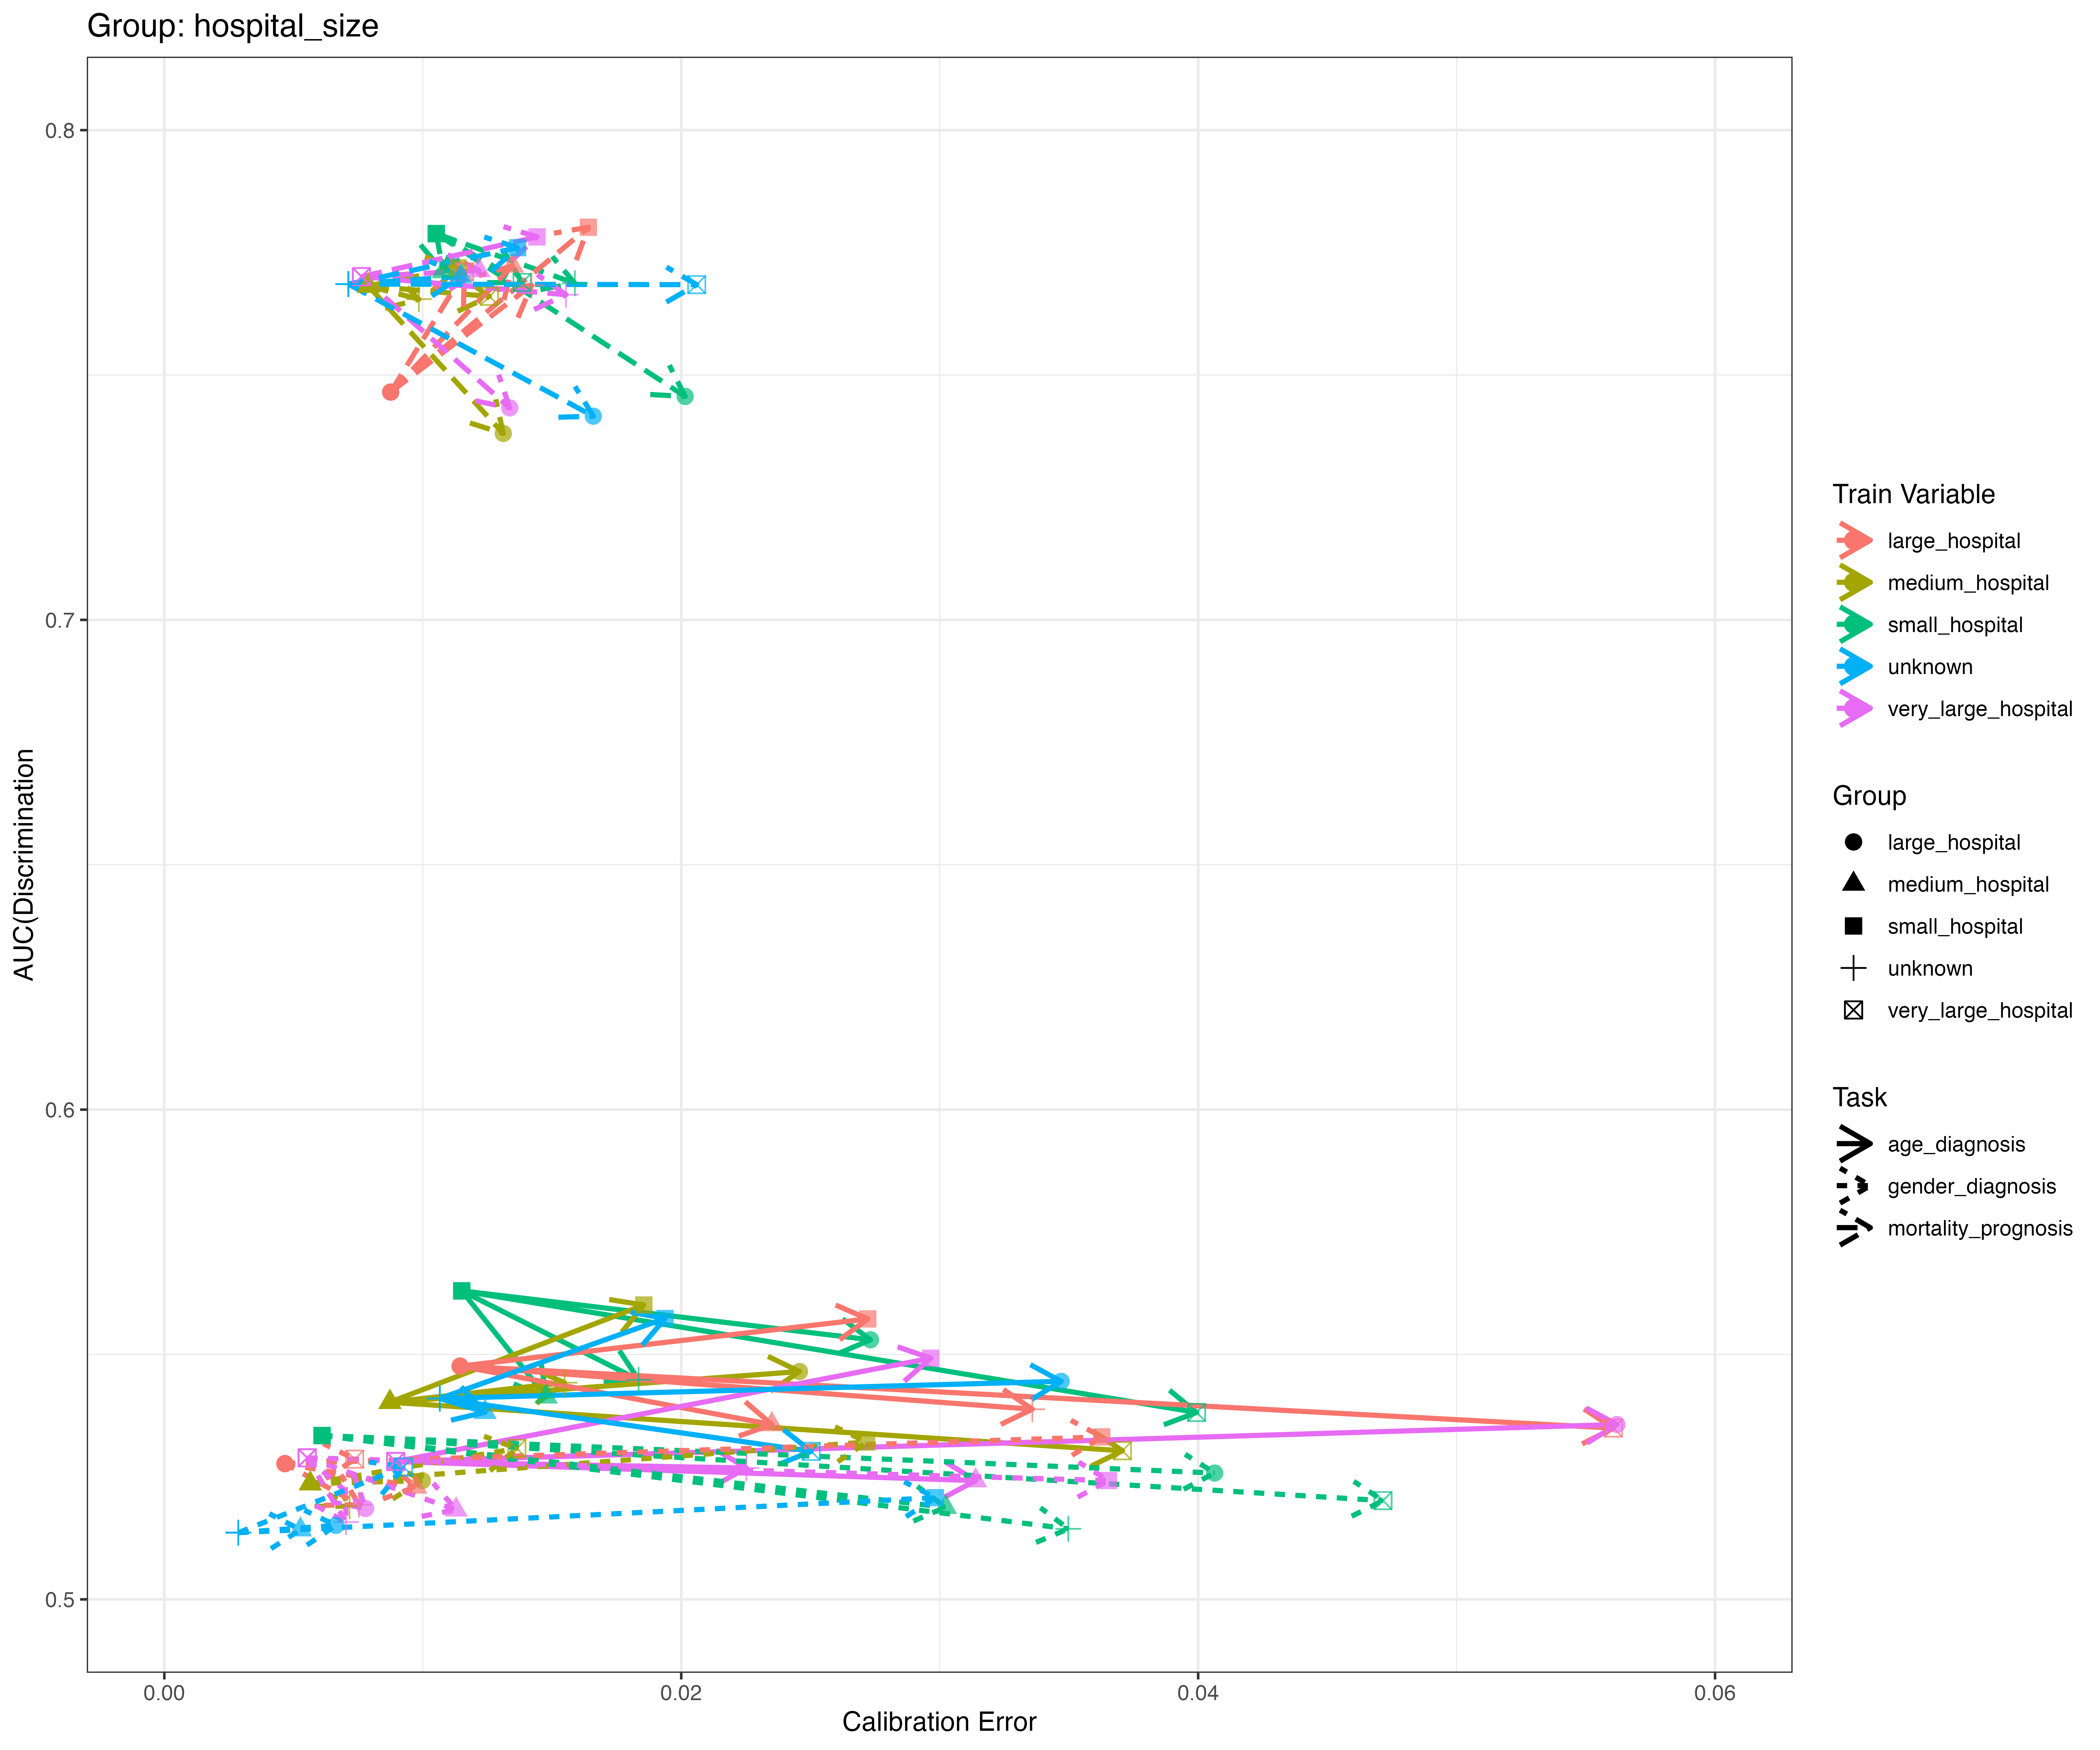
\includegraphics[height=0.45\textheight]{./figures/figure2.png}  % 图像2,设置高度
  \caption{Discrimination vs. Calibration Error Across Hospital Sizes and Tasks.}
  \label{fig:figure2}
\end{minipage}

\vspace{1cm}  

\begin{minipage}{\textwidth}
  \centering
  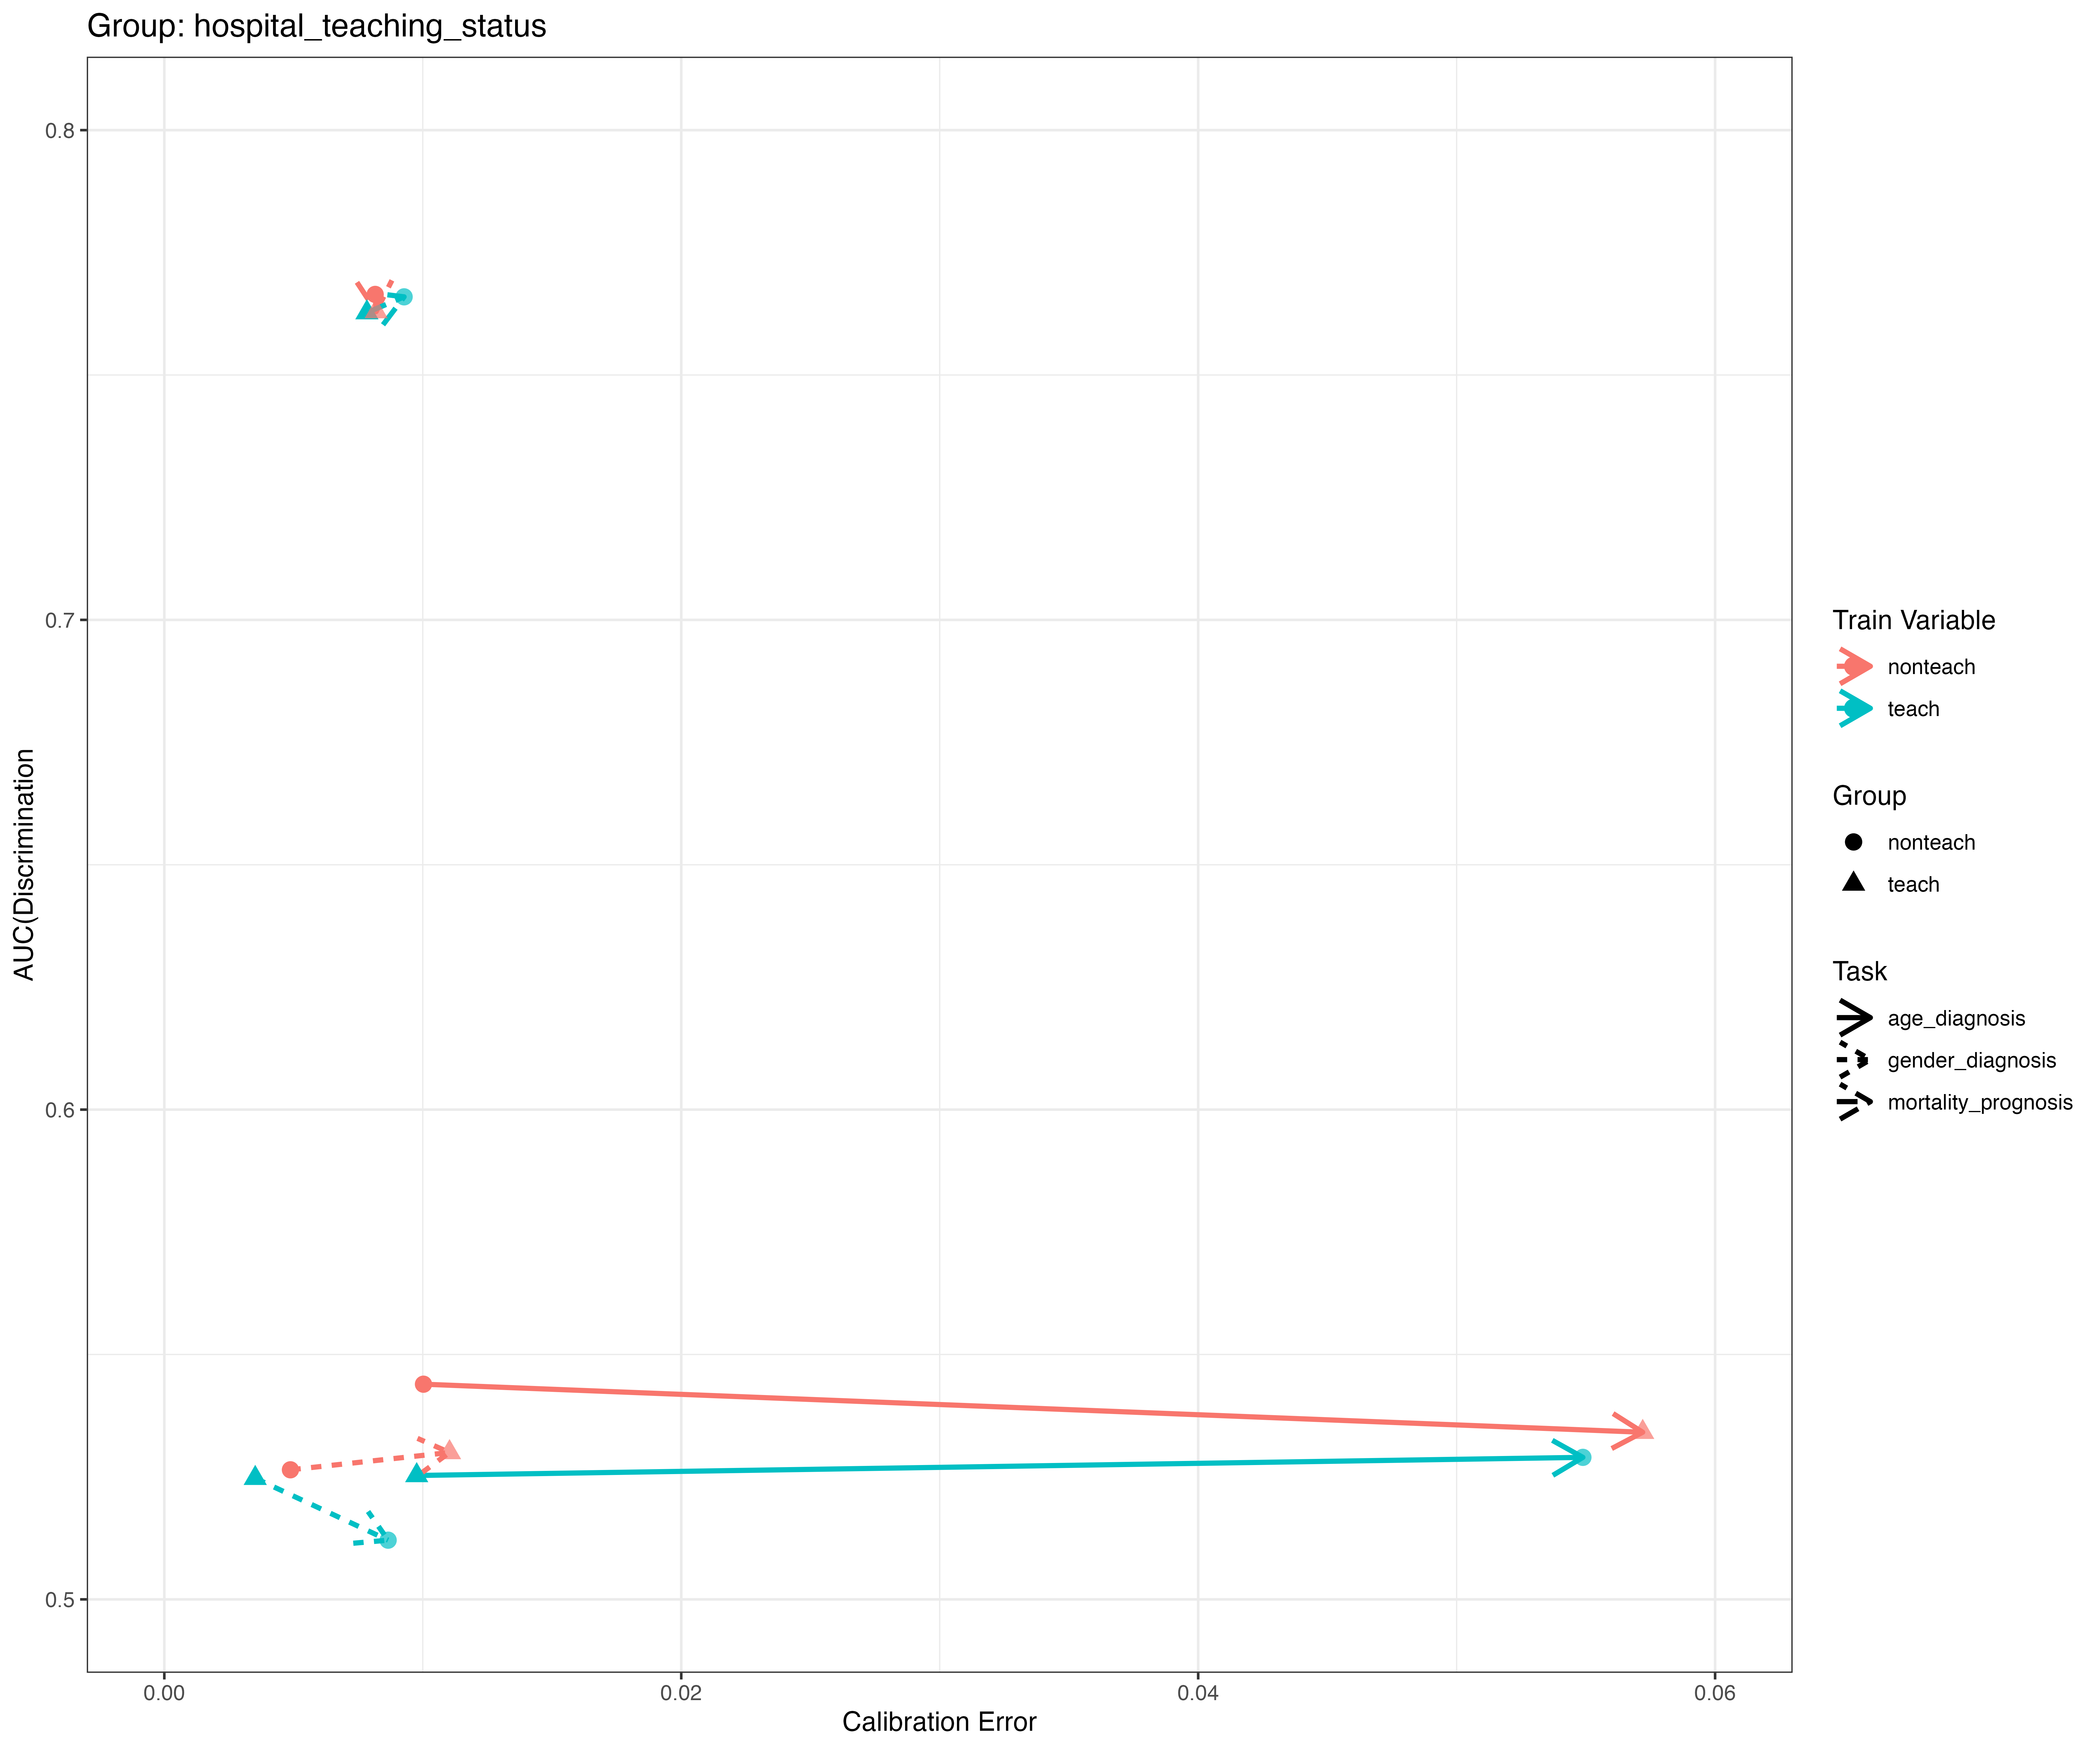
\includegraphics[height=0.45\textheight]{./figures/figure3.png}  % 图像3,设置高度
  \caption{Discrimination vs. Calibration Error Across Hospital Teaching Status and Tasks.}
  \label{fig:figure3}
\end{minipage}
\end{figure}


\clearpage
%==============================
\newpage
\section{Discussion}\label{discussion}
%==============================

The study aims to empirically validate that calibrations stay consistent for causal-direction (prognostic) models while discriminations remain stable for anti-causal (diagnostic) models under case-mix shift. Our findings partly support this hypothesis, as the calibration errors of the mortality prognostic model remain consistent across the training and test settings. 
  
In Figures 1-3, the mortality prognostic model demonstrates robust and reliable performance across varying subgroups, with consistently high AUC values ranging from 0.75 to 0.8 and small calibration errors.  The short arrow lengths and consistent directions indicate small variability between the training and testing sets, confirming the hypothesis that prognostic models maintain stability under external validation.  The well-calibrated performances on both the training sets and the test sets are likely due to the predictors in the model covering comprehensive and multidimensional patients’ physiological information that reduce the impact of confounding factors, thus ensuring robust performance under shift in case-mix. In contrast, Age diagnosis and gender diagnosis have low AUC values (0.5-0.6), reflecting unreliable results that lack strong comparative significance. The unsatisfactory performance may be due to the limited and unrepresentative predictors that fail to capture enough information for class distinction. 
  
The current study includes only three tasks, and the low AUC value (0.5- 0.6) indicates the unreliability of the two diagnostic models, making them insufficient to support further analysis. Future work will focus on training more tasks and selecting appropriate predictors. Considering the results based on figures alone are not rigorous, we will use statistical tests to assess whether the variances of calibration and discrimination between the training fold and test fold differ significantly across prognostic and diagnostic models.

\newpage
%==============================
\bibliographystyle{vancouver}
\bibliography{literature}
%==============================

\end{document}